\chapter{Capítulo 2}
Existen varias normas para la citación bibliográfica. Algunas áreas del conocimiento prefieren normas específicas para citar las referencias bibliográficas en el texto y escribir la lista de bibliografía al final de los documentos. Esta plantilla brinda la libertad para que el autor de la tesis  o trabajo de investigación utilice la norma bibliográfica común para su disciplina. Sin embargo, se solicita que la norma seleccionada se utilice con rigurosidad, sin olvidar referenciar "todos" los elementos tomados de otras fuentes (referencias bibliográficas, patentes consultadas, software empleado en el manuscrito, en el tratamiento a los datos y resultados del trabajo, consultas a personas (expertos o público general), entre otros).\\

\section{Ejemplos de citaciones bibliográficas}
Existen algunos ejemplos para la citación bibliográfica, por ejemplo, Microsoft Word (versiones posteriores al 2006), en el  menú de referencias, se cuenta con la opción de insertar citas bibliográficas utilizando la norma APA (American Psychological Association) u otras normas y con la ayuda para construir automáticamente la lista al final del documento. De la misma manera, existen administradores bibliográficos compatibles con Microsoft Word como Zotero, End Note y el Reference Manager,  disponibles a través del Sistema Nacional de Bibliotecas (SINAB) de la Universidad Nacional de Colombia\footnote{Ver:www.sinab.unal.edu.co } sección "Recursos bibliográficos" opción "Herramientas Bibliográficas. A continuación se muestra un ejemplo de una de las formas más usadas para las citaciones bibliográficas.\\

Citación individual:\cite{AG01}.\\
Citación simultánea de varios autores:
\cite{AG12,AG52,AG70,AG08a,AG09a,AG36a,AG01i}.\\

Por lo general, las referencias bibliográficas correspondientes a los anteriores números, se listan al final del documento en orden de aparición o en orden alfabético. Otras normas de citación incluyen el apellido del autor y el año de la referencia, por ejemplo: 1) "...énfasis en elementos ligados al ámbito ingenieril que se enfocan en el manejo de datos e información estructurada y que según Kostoff (1997) ha atraído la atención de investigadores dado el advenimiento de TIC...", 2) "...Dicha afirmación coincide con los planteamientos de Snarch (1998), citado por Castellanos (2007), quien comenta que el manejo..." y 3) "...el futuro del sistema para argumentar los procesos de toma de decisiones y el desarrollo de ideas innovadoras (Nosella \textsl{et al}., 2008)...".\\

\section{Ejemplos de presentación y citación de figuras}
Las ilustraciones forman parte del contenido de los capítulos. Se deben colocar en la misma página en que se mencionan o en la siguiente (deben siempre mencionarse en el texto).\\

Las llamadas para explicar algún aspecto de la información deben hacerse con nota al pie y su nota correspondiente\footnote{Las notas van como "notas al pie". Se utilizan para explicar, comentar o hacer referencia al texto de un documento, así como para introducir comentarios detallados y en ocasiones para citar fuentes de información (aunque para esta opción es mejor seguir en detalle las normas de citación bibliográfica seleccionadas).}. La fuente documental se debe escribir al final de la ilustración o figura con los elementos de la referencia (de acuerdo con las normas seleccionadas) y no como pie de página. Un ejemplo para la presentación y citación de figuras, se presenta a continuación (citación directa):\\

Por medio de las propiedades del fruto, según el espesor del endocarpio, se hace una clasificación de la palma de aceite en tres tipos: Dura, Ternera y Pisifera, que se ilustran en la Figura
\ref{fig:Fruto}.\\
\begin{figure}
\centering%
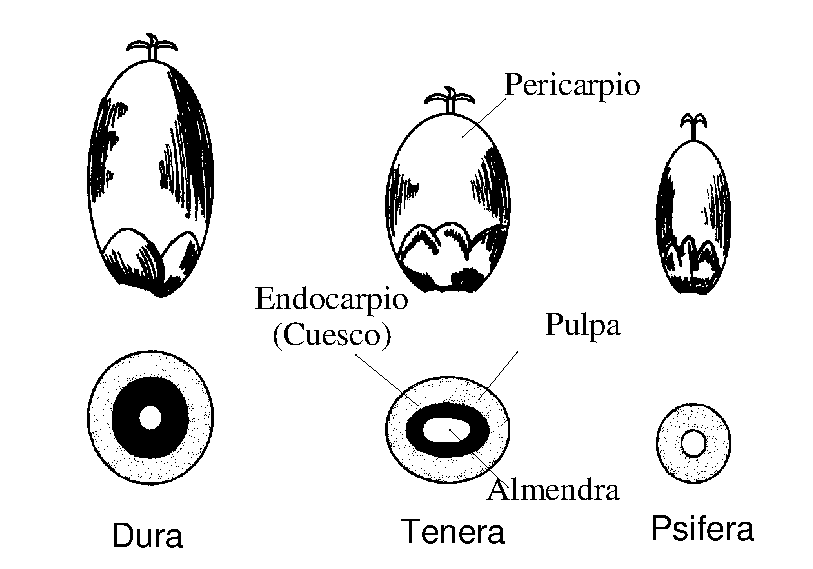
\includegraphics{Kap3/FrutoSp}%
\caption{Tipos y partes del fruto de palma de aceite \cite{AG03p,AG04p}.} \label{fig:Fruto}
\end{figure}

\section{Ejemplo de presentación y citación de tablas y cuadros}
Para la edición de tablas, cada columna debe llevar su título; la primera palabra se debe escribir con mayúscula inicial y preferiblemente sin abreviaturas. En las tablas y cuadros, los títulos y datos se deben ubicar entre líneas horizontales y verticales cerradas (como se realiza en esta plantilla).\\

La numeración de las tablas se realiza de la misma manera que las figuras o ilustraciones, a lo largo de todo el texto. Deben llevar un título breve, que concreta el contenido de la tabla; éste se debe escribir en la parte superior de la misma. Para la presentación de cuadros, se deben seguir las indicaciones dadas para las tablas.\\

Un ejemplo para la presentación y citación de tablas (citación indirecta), se presenta a continuación:\\

De esta participación aproximadamente el 60 \% proviene de biomasa
(Tabla \ref{EMundo1}).
\begin{center}
\begin{threeparttable}
\centering%
\caption{Participación de las energías renovables en el suministro
total de energía primaria \cite{AG02i}.}\label{EMundo1}
\begin{tabular}{|l|c|c|}\hline
&\multicolumn{2}{c|}{Participación en el suministro de energía primaria /\% (Mtoe)\;$\tnote{1}$}\\\cline{2-3}%
\arr{Región}&Energías renovables &Participación de la biomasa\\\hline%
Latinoamérica&28,9 (140)&62,4 (87,4)\\\hline%
\:Colombia&27,7 (7,6)&54,4 (4,1)\\\hline%
Alemania&3,8 (13,2)&65,8 (8,7)\\\hline%
Mundial&13,1 (1404,0)&79,4 (1114,8)\\\hline
\end{tabular}
\begin{tablenotes}
\item[1] \footnotesize{1 kg oe=10000 kcal=41,868 MJ}
\end{tablenotes}
\end{threeparttable}
\end{center}

NOTA: en el caso en que el contenido de la tabla o cuadro sea muy extenso, se puede cambiar el tamaño de la letra, siempre y cuando ésta sea visible por el lector.\\

\subsection{Consideraciones adicionales para el manejo de figuras y tablas}
Cuando una tabla, cuadro o figura ocupa más de una página, se debe repetir su identificación numérica, seguida por la palabra continuación.\\

Adicionalmente los encabezados de las columnas se deben repetir en todas las páginas después de la primera.\\

Los anteriores lineamientos se contemplan en la presente plantilla.\\

\begin{itemize}
\item Presentación y citación de ecuaciones.
\end{itemize}

La citación de ecuaciones, en caso que se presenten, debe hacerse como lo sugiere esta plantilla. Todas las ecuaciones deben estar numeradas y citadas dentro del texto.\\

Para el manejo de cifras se debe seleccionar la norma según el área de conocimiento de la tesis  o trabajo de investigación.\\